\chapter{The project: MongoDB Performance}
\label{cha:3}
In this chapter the real core of this research, the project \textsc{MongoDB Performance}, is presented starting with the analysis  that we made before developing the software that consequently decreed the implementation choices.
Following there is an overview on the frameworks used and in the end the whole application is described in depth also showing screenshots of the user interface.

\section{Aim of the project and beginning idea}
\label{sec:1}
When benchmarking a product, the standard procedure is to compare it with its competitors, but in this case it took a while to the company to decide which kind of analysis could better fit the availability of time and money.
The beginning idea was in fact to build a software able to perform a stress test on different database technologies, and then to compare those tests and choose the one who could best support the requirements.
Technologies taken in account where MongoDB, Apache Cassandra and PostgreSQL with JSON datatype \footnote{https://www.postgresql.org/docs/9.6/static/datatype-json.html}, but after a meeting with the customer we decided to choose one technology for a specific test using as measurement parameters many benchmarks found on the web and the declared specifications, ease of use and configuration.
PostgreSQL was discarded almost immediately due to lower performance confirmed by third part benchmarks, so MongoDB became the first choice thanks to its simplicity and Cassandra was left as second choice in case Mongo couldn’t satisfy the requirements, even if it seemed to have better results on most of the benchmarks found on the Web. 
As mentioned, the customer gave us specific necessities:
\begin{itemize}
	\item The software counts many hundred thousands of active users with thousands of records each one, so the database should be able to support several millions of total records.
	\item It works as a web application and needs to be responsive to give the user the best usage experience,consequently it should query results in no more than 2 seconds.
	\item It contains important billing information, so data cannot be lost.
	\item The web application is online 24/7 and it can be stopped only when releasing a new version. So even in the time slots with more expected traffic, any system crash must be prevented.
\end{itemize}
The final aim of the project so is not a benchmark between different DMBS, but a specific one performed on the chosen technology with the possibility to be eventually extended to other solutions.


\section{Implementation choices and architecture}
\label{sec:2}
It became clear that the beginning idea of a complete benchmark over the most used DBMS was impossible in term of time and money costs.
I decided to develop a modular application following the patterns of microservices. Due to this choice, the final result allows to reuse a good part of the software  adding a new module for each eventual DMBS, using the existing code from the MongoDB module and adapting it to another database technology with the proper drivers provided by Java Spring.
In the end thanks to the satisfactory results obtained by MongoDB, there was no need to include other technologies in the benchmark.
\newpage
The architecture, drawed with \textit{Draw.io} \footnote{https://www.draw.io}, presents  both the implemented modules and the possible or discarded modules (dot-line) to give an overview of how a microservices production application should look
Due to time issues, we decide to not implemented all unnecessary modules like for example the \textit{Authentication Module}.
\begin{figure}
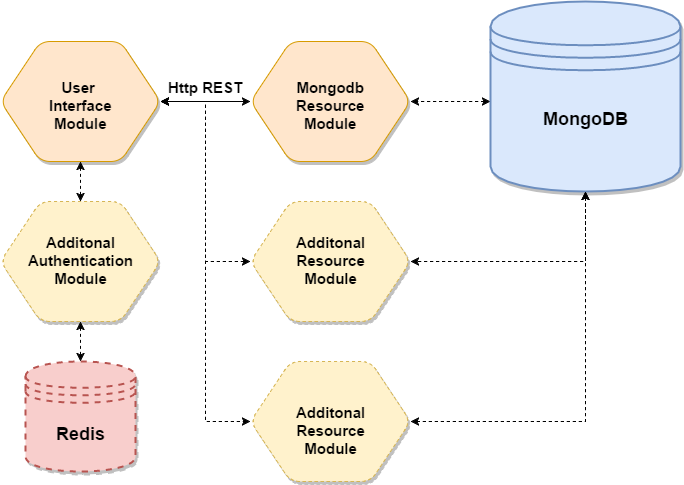
\includegraphics[scale=0.5]{app-architecture.png}
\centering
\caption{Rappresentation of the architecture including possible future implementations}
\end{figure}



\section{Java Spring and AngularJS}
\label{sec:3}
\textsc{Spring} framework has become over the years one of the most popular Java frameworks for building  Enterprise applications, becoming an alternative (or replacement) for the more classical Enterprise Java Beans (EJB)  \footnote{https://en.wikipedia.org/wiki/Enterprise\_JavaBeans}. It introduced the concept of \textit{aspect-oriented} programming that is a programming paradigm that aims to increase modularity by allowing the separation of cross-cutting concerns. It’s composed by many modules, including Spring Security for authorization and authentication, Spring Web for customization of web applications using RESTful web services and Spring Data Access working with \textsc{JDBC} \footnote{http://www.oracle.com/technetwork/java/javase/jdbc/index.html} and object-relational mapping tools to support both relational and NoSQL databases. 
It can create standalone “runnable” production-grade applications with Spring Boot, including an embedded Tomcat, and opinionated \textit{POMs} \footnote{https://maven.apache.org/guides/introduction/introduction-to-the-pom.html} to simplify Maven configuration and production-ready features.
Those features, such as metrics, health check togheter with externalized configuration make it the definitive framework for Java Web applications among the java developer community and  it immediately became my unquestionable choice thanks to its affinity to micro-services model.
On the front-end side, AngularJS was the perfect choice thanks to its natural affinity with Spring and Twitter Bootstrap and its routing management system for dynamic loading dynamic content inside single-page applications. I’ve chosen version 1.6 instead of the new version AngularJS 2, that has a different and more complex implementation and usage based on TypeScript, and I’ve made a wide use of it especially in the User Interface Module that manages the launch and data plotting  of the stress-test.

\section{Microservices and modularity}
\label{sec:4}

\section{Final modules and possible implementations}
\label{sec:5}

\subsection{Architecture of the application}
The architecture was designed to be reusable and extensible following the theory of microservices. That’s why it was way more complex than the final result, with more modules each dedicated to provide a single functionality. The first design provided the following modules:
\begin{itemize}
	\item \textit{User Interface Module} : it has been kept in the final application and its functionality is related to serve the web resources that compose the front end of the application
	\item \textit{Authentication Module} : it was in beginning implemented and then removed because of possible usage compolexity and also because of no real use during the main test. This module was connected to a \textsc{Redis} \footnote{https://redis.io} instance, that is a NoSQL database of key-value type with semi-persistence of the data through snapshots and was used to store the tokens to authenticate users of the application. Since there was need for only one user (me, as admin), the authentication service has been rewritten as angular module \textit{auth.js} for a single user inside the \textit{User Interface Module}. Anyway, it is still possible to add this module to the application for further usages in the future, as it is good practice too keep separated authentication from other functionalities.
	\item \textit{MongoDB Resource Module} : is the main module that connects to MongoDB and its functionality is related to perform all the tasks needed for the stress test.
	\item \textit{Additional Resource Modules} : these modules are all the\textit{n} modules siblings of \textit{MongoDB Resource Module} that could possibly be implemented to support different DBMS for the application. None of them have been actually realized and I decided to show only two in the schema as reminder for the possibilities taken into account at the beginning of the project but discarded for the motivations explained in chapter 2, Apache Cassandra and PostgreSQL with JSON datatype
\end{itemize}

\subsection{User Interface module}

\subsection{MongoDB Resource module}